\chapter{Background}
\label{cha:background}
This thesis investigates a middleware for de-identifying data exposed through the Solid protocol. Section \ref{sec:solid} introduces the basic concepts of Solid, while section \ref{sec:pets} introduces some necessary background knowledge on \gls{PETs}.

\section{Solid}
\label{sec:solid}

\subsection{Introduction}
\begin{quote}{Tim Berners-Lee}
    The Semantic Web is not a separate Web but an extension of the current one, in which information is given well-defined meaning, better enabling computers and people to work in cooperation.
\end{quote}

\noindent In 2001, Sir Tim Berners-Lee - the inventor of the world-wide web - published an article in \textit{Scientific American} entitled `The semantic Web' \citep{semantic-web}. It envisioned a future where the Web was not just a collection of pages with meaningless links to each other, but a smart Web, where objects have well-defined meanings.

Today, most resources accessible on the Web are meant for people to read, understand and process, but it is not adapted to automated processing by software agents. Computers can read information and format it correctly, but they lack a unified way to interpret the information: there is no way to process the \textit{semantics}. The Semantic Web tries to solve this problem by extending the current Web with new, compatible standards and protocols to attach computer-readable meaning to information available on the Web.

Currently, markup languages such as XML enable users to arbitrarily structure documents the way they want it (e.g. using a tag called \texttt{<book>} and a tag called \texttt{<isbn>}). They then write software that parses this by telling the software that \texttt{<book>} means "book" and \texttt{<isbn>} means "isbn". However, other users may use different terms (e.g. \texttt{<livre>}), making information not universally parsable. 

\noindent The Semantic Web introduces the \gls{RDF}, which encodes structure and information in sets of triples: a subject, a predicate and an object. These triples  then create a knowledge graph called an RDF graph, where predicates relate subjects to objects. The objects in one triple can then be the subjects in another one. The figure below illustrates an example, where Tokyo is the subject of a linked data triple, and two predicates relate it to its area and the country it resides in. The object, Japan, may then be the subject of other RDF graphs, relating it for example to its population.

\begin{figure}[H]
    \centering
    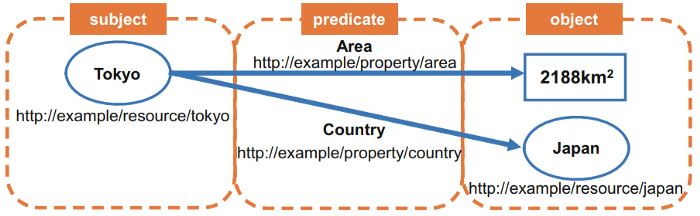
\includegraphics[width = 0.9\textwidth]{images/background/linked-data.png}
    \caption{\gls{RDF} representation of the city Tokyo, with predicates relating it to its area and its country. Source: \citet{generating-pva}}
    \label{fig:linked-data}
\end{figure}

\noindent Subjects, predicates and objects are all identified by a URI, making them universal, and allowing anyone to define new predicates\footnote{Unless they are literals, such as the area in the example}. Like this, webs of information are formed between related objects using definitions that can be found and understood by everyone.

This does not completely solve the problem, however. It is possible that multiple definitions exist for essentially the same object. To resolve this, the Semantic Web introduces a third component: ontologies. Ontologies are documents that formally define the relations among terms \citep{semantic-web}. A widely-used ontology is called \textit{foaf}\footnote{\url{ http://xmlns.com/foaf/spec/}} (friend-of-a-friend): it is used to describe relationships between people.

\gls{RDF}, however, is only something conceptual (a collection of subject, predicate and object). If we want to actually use it, we need to store \gls{RDF} in documents. This is possible in multiple ways, i.e., multiple representation formats exist. The most popular ones are Turtle \citep{turtle} and JSON-LD \citep{jsonld}. Turtle has the advantage that it allows you to define prefixes at the top of the file, which are aliases for the long URIs that you use to relate the subjects/predicates/objects. If you want to talk about the foaf ontology, you can define at the top of your file:

\texttt{@prefix foaf <http://xlmns.com/foaf/0.1/>}

\noindent You can then use \texttt{foaf} in the rest of your turtle file, instead of \texttt{<http://xlmns.com/\\foaf/0.1/>}. This makes it very human-readable compared to other formats. Additional existing formats are \gls{RDF}/XML and N-Triples, but they are less common.

\subsection{The Solid Protocol}
\begin{quote}{\href{https://solidproject.org}{solidproject.org}}
    Solid is a proposed set of conventions and tools for building \textit{decentralized applications} based on Linked Data principles.
\end{quote}
\noindent Solid \citep{solid} is a proposed W3C specification that wishes to decentralize the web by giving people control over their data. Solid aims to realize this by giving people an online datastore called a \textit{pod} (personal online datastore). Users can then login to applications using an authentication mechanism provided by Solid, and the application can in turn access data stored in the user's pod.

By storing all the data inside the user's pod instead of on the application server, the user retains complete control over his data. He can flexibly choose what data to share with what applications. Furthermore, storing the data in a pod reduces vendor lock-in: when the user wishes to switch from one service to another, he can simply give the new application access to the data he already possesses. 
In Solid, there are two types of resources: linked and non-linked data resources. Non-linked data resources are the usual kinds of data that we access on the web right now (binary, text, images, ...), while linked data follows the 
 \gls{RDF} specifications by using a content representation such as Turtle. These linked-data standards follow the principles of the Semantic Web.

\subsection{Authentication}
Authenticating a user is the act of verifying a user's claimed identity. Identities in solid (both for users and other agents) follow the WebID standard \citep{webid}: URIs act as universal identifiers. An example WebID is:

\begin{center}
   \texttt{https://jessegeens.solidcommunity.net/profile/card\#me}\\
\end{center}

\noindent These WebID URIs can identify several things: users, software agents, or other things (even if they do not exist on the web). The WebID URI references a WebID Profile Document. This document contains information about the agent who is the referent of the WebID URI. However, an important distinction must be made. When the \textit{\texttt{\#me}} is included in the URI (or more in general, the hashtag), this URI refers to an agent. When the hashtag is omitted, the URI refers to the document describing this agent.

While the WebID standard provides identities, it does not yet verify them. The actual authentication (or, verifying that the agent actually controls the WebID he claims to control) in Solid uses the WebID-OIDC protocol. This protocol draws inspiration from OAuth2 and from OpenID Connect. The below workflow, drawn from the WebID-OIDC repository, explains the basic mechanism of the protocol:

\todo{Also here, make sure this is not plagiarism, since it is copied from the repo}

\begin{quote}{\href{https://github.com/solid/webid-oidc-spec}{webid-oidc-spec repository}}

    1. \textbf{Initial Request}: Alice (unauthenticated) makes a request to bob.example, receives a \texttt{HTTP 401 Unauthorized} response, and is presented with a 'Sign In With...' screen.\\
    
    2. \textbf{Provider Selection}: She selects her WebID service provider by clicking on a logo, typing in a URI (for example, alice.solidtest.space), or entering her email.\\
    
    3. \textbf{Local Authentication}: Alice gets redirected towards her service provider's own Sign In page, thus requesting https://alice.solidtest.space/signin, and authenticates using her preferred method (password, WebID-TLS certificate, FIDO 2 / WebAuthn device, etc).\\
    
    4. \textbf{User Consent}: (Optional) She's presented with a user consent screen, along the lines of "Do you wish to sign in to bob.example?".\\
    
    5. \textbf{Authentication Response}: She then gets redirected back towards https://bob.example/resource1 (the resource she was originally trying to request). The server, bob.example, also receives a signed ID Token from alice.solidtest.space that was returned with the response in point 3, attesting that she has signed in.\\
    
    6. \textbf{Deriving a WebID URI}: bob.example (the server controlling the resource) validates the ID Token, and extracts Alice's WebID URI from inside it. She is now signed in to bob.example as user https://alice.solidtest.space/\#i.\\
    
    7. \textbf{WebID Provider Confirmation}: bob.example confirms that solidtest.space is indeed Alice's authorized OIDC provider (by matching the provider URI from the iss claim with Alice's WebID).

\end{quote}

\subsection{Authorization}
Authorization within the Solid project builds on the Web Access Control standard \citep{wac}. The WAC standard provides a method to define authorization conditions for resources in a Pod using an \gls{ACL}.\todo{Explain here what an access control list is?} Every resource is coupled with an \gls{ACL} resource - either directly, or by inheriting it from a parent container. These \gls{ACL} resources are using the ACL ontology, usually in a turtle file\footnote{Other \gls{RDF} representations are also allowed, but support for turtle files is mandatory}. Authorization conditions consist of three elements: access objects (the associated resource), access modes (\textit{read}, \textit{write}, \textit{append} or \textit{control}) and access subjects (the agents performing the request).

The access objects in an \gls{ACL} resource are the resources the \gls{ACL} resource refers to. This can be both a normal resource (LDP-RS or LDP-NR, see \ref{subsec:ldp}) as well as a container. It is not mandatory for resources to have an associated ACL resource, as these can be inherited. This mechanism ensures that there is no need to create duplicate ACL resources for similar resources, as well as ensuring proper protection for newly created resources. When a resource is accessed, the server will first look for a directly associated \gls{ACL} resource. When none is found, the server will walk up the container tree (starting from the current container the resource is located in, then the parents, up until the root container). Once an \gls{ACL} resource applying to one of the parent containers is found, this is applied to the requested resource.

Possible access modes, then, are either \textit{read}, \textit{write}, \textit{append} or \textit{control}. Reading and writing are the usual operations. Append is a subset of writing: data can be added to the resource, but not deleted. This is useful for, for example, logging applications, ensuring that logs cannot be removed. Since appending is a subset of writing, the writing authorization implies the appending authorization (no resource can allow writing but disallow appending). Finally, control means being able to modify the ACL of the resource. Being able to control a resource generally implies ownership of the resource.

Lastly, access subjects are those agents who request a certain operation on the resource. Generally, these can be divided into four categories. The first one is \textit{every agent}, i.e., the resource is publicly accessible. A second option is authenticated agents only (with no restrictions on who these agents are), which may be useful for auditing purposes. Thirdly, resource access can be restricted to agents with a specific WebID. Finally, this can also be extended to groups of agents (where the group has a single WebID). An example \gls{ACL} resource, taken from the Solid Community Server\footnote{See \url{https://github.com/solid/community-server}}, is presented below:
\lstinputlisting[style=turtle, title=.acl, caption=Access Control List Resource]{code/acl.ttl}

\subsection{Linked Data Platform and Containers}
\label{subsec:ldp}
Solid mainly relies on the \gls{LDP} protocol \citep{ldp} for resource management. The \gls{LDP} protocol uses HTTP for accessing and modifying resources on a server. LDP Resources, or LDPRs, are HTTP resources that conform to a number of conventions. There are multiple types of resources:
\begin{enumerate}
    \item \gls{RDF} Sources, also called LDP-RSs (LDP \gls{RDF} Source)
    \item Non-\gls{RDF} Sources, such as images or binary data, which are called LDP-NRs
    \item Containers, a concept for bundling related resources together. These are also called LDPCs (LDP Container). 
\end{enumerate}

\noindent To support the access and modification of these resources, \gls{LDP} servers must support a number of HTTP methods on the resources. The \texttt{GET} method is mandatory and returns the request resource, if certain conditions are met (e.g., does the agent have the correct authorizations to access the resource). The \texttt{POST} and \texttt{PUT} methods are optional, and allow agents to create new resources or modify existing ones. Similarly, the \texttt{DELETE} method is optional and allows agents to delete resources. The \texttt{HEAD} and \texttt{OPTIONS} methods are mandatory to be implemented by servers and are similar to the methods defined in the HTTP/1.1 protocol. Below is an example of a request for a basic container and the accompanying reply \citep[from][]{ldp-primer}:

\begin{verbatim}
GET /alice/ HTTP/1.1
Host: example.org
Accept: text/turtle
HTTP/1.1 200 OK 
Content-Type: text/turtle; charset=UTF-8
Link: <http://www.w3.org/ns/ldp#BasicContainer>; rel="type", 
      <http://www.w3.org/ns/ldp#Resource>; rel="type"
Allow: OPTIONS,HEAD,GET,POST,PUT,PATCH
Accept-Post: text/turtle, application/ld+json, image/bmp, image/jpeg
Accept-Patch: text/ldpatch
Content-Length: 250
ETag: W/'123456789'
	
@prefix dcterms: <http://purl.org/dc/terms/>.
@prefix ldp: <http://www.w3.org/ns/ldp#>.
	
<http://example.org/alice/> a ldp:Container, ldp:BasicContainer;
  dcterms:title 'Alice`s data storage on the Web' .	
\end{verbatim}

\newpage
\begin{formal}
\textbf{Optional reading} $ - $
\textit{LDP Containers}\\

\noindent LDP Containers are a specialization of a LDP \gls{RDF} Source, which represent a set of links to other LDPRs that are contained within the container. There are multiple types of LDPCs. The simplest one is the Basic Container or LDP-BC. It defines a basic notion of containment using a generic vocabulary and a \texttt{ldp:contains} relationship. In LDP-BCs, there are no restrictions on LDPRs contained within. The figure below illustrates a LDP Basic Container.\\
\phantom{kkkkkkkkk||||||}{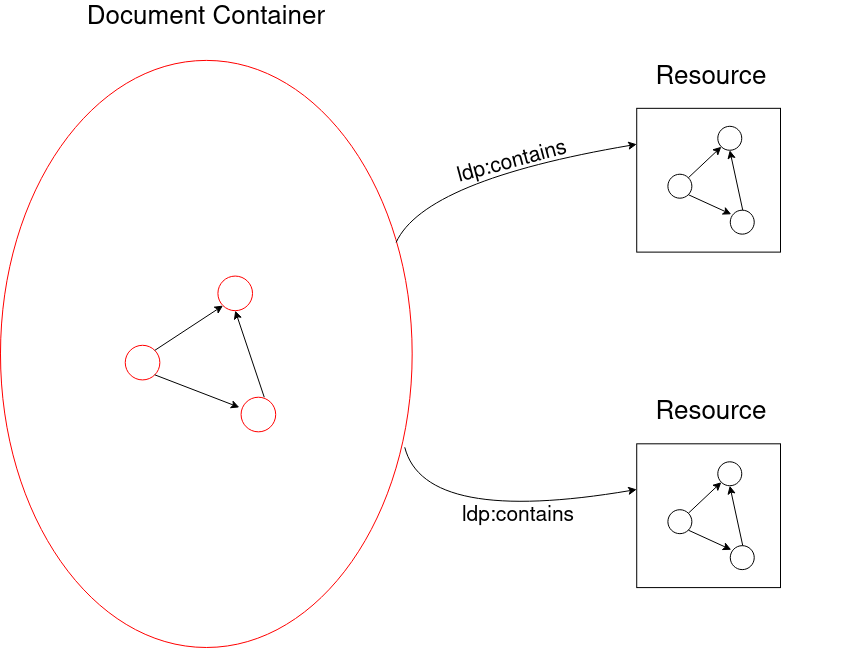
\includegraphics[width=0.60\textwidth]{images/background/ldp-bc.png}}\\
\noindent Direct Containers, or LDP-DCs, are a specialization of a Basic Container. The LDP-DC can make assertions, called membership triples, on resources withing the container. These assertions, which use domain-specific vocabulary, are made as part of the creation process for resources placed in the container. The membership triples do not need to refer to the container resource - these can refer to other resources as well. The figure below illustrates a LDP Basic Container containing movies, and a LDP Direct Container containing documents (images, movies, ..) where the actor is depicted, illustrated through the predicate \texttt{foaf:depicton}. \\
\phantom{kkk|||}{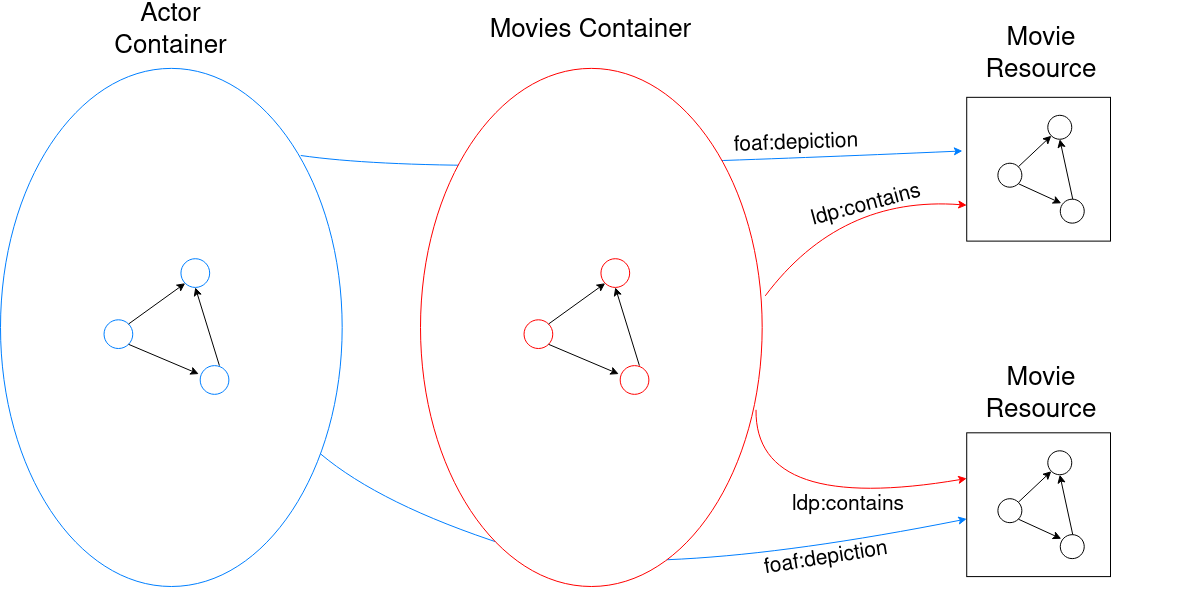
\includegraphics[width=0.9\textwidth]{images/background/ldp-dc.png}}\\

\noindent \textit{Source}: \url{https://www.w3.org/TR/ldp-primer/}
\end{formal}

\newpage
\section{Privacy-Enhancing Technologies}
\label{sec:pets}
\subsection{The need for Privacy-Enhancing Technologies}
The concept of privacy has been around for a long time. Even in the 14th century already, cases were brought before court for eavesdropping and opening letters \citep{privacy-history}. Initially, it was more understood in the context of being let alone, especially in one's house or personal properties. Since the dawn of the information age after the Second World War, the concept started to shift more towards privacy in the context of personal information and publications on the topic started to appear. The definition did not change much however, remaining very similar to the one introduced in 1891 by Warren and Brandeis \citep{privacy-history}:
\begin{quote}{Samuel Warren, Louis Brandeis}
    Privacy is described as a right to be let alone and a right of each individual  to  determine,  under  ordinary  circumstances,  what  his  or  her  thoughts, sentiments, and emotions shall be when in communication with others.
\end{quote}
\todo{Compare with definition of privacy in introduction to PETs, compare inward and outward definition}
\noindent The ubiquity of personal data collection in recent years has strengthened privacy concerns. Especially since the Web has become extremely centralized, with only six companies accounting for 43\% of global internet traffic \citep{internet-report}, there has been a growing demand for technologies that help protect user privacy.

Not only from the data subject's perspective is there a growing concern for data privacy. With the introduction of the \gls{GDPR} in 2018, companies have a legal obligation to take care of user data, especially if it is sensitive. This clashes with the rise of the Saas/PaaS business models, where companies outsource data storage and management. However, this is not always possible and comes with risks. If a Data Processor (a third party that processes data on behalf of a Data Controller) leaks data, the Data Controller risks violating the user's trust (and legal sanctions). \todo{Optional reading or subsection about GDPR to explain basics and terminology?}

In both cases, Privacy-Enhancing Technologies play a big role in reducing the risk of data leaks and preserving user privacy. \citeauthor{pets-handbook} introduced the following definition, which was later adopted by the European Commission\footnote{\url{https://eur-lex.europa.eu/LexUriServ/LexUriServ.do?uri=COM:2007:0228:FIN:EN:PDF}}:
\begin{quote}{\citeauthor{pets-handbook}}
    Privacy-Enhancing Technologies is a system of ICT measures protecting informational privacy by eliminating or minimising personal data thereby preventing unnecessary or unwanted processing of personal data, without the loss of the functionality of the information system.
\end{quote} 
The following sections will introduce a number of widely used \gls{PETs}, some of which will be used in \middleware{}.

\subsection{Data (de-)identification}
\label{sec:data-deid}
The previous section gave an introduction to the concept of privacy. In IT systems, this applies to personal data. But when is data personal? In the context of ePrivacy, the term \textit{\gls{PII}}, is used widely. The term applies to data elements that contain references to attributes that can, either directly or indirectly, disclose someone's identity. A distinction can then be made between three types of data \citep{de-id-taxonomy}:
\begin{itemize}
    \item \textbf{Direct identifiers}: data attributes that directly identify an individual. Examples are national identification numbers, home addresses, e-mail addresses, full names, etc.
    \item \textbf{Indirect identifiers}: data attributes that can be combined with other data attributes to identify an individual, but do not disclose an identity on their own. Examples are birth dates, family names, IP addresses etc.
    \item \textbf{Non-PII elements}: data attributes that contain no reference at all to a person's identity.
\end{itemize}
\noindent \citeauthor{privacy-design-strategies} notes that much like security, privacy is a core property of software systems, and is heavily architecture-dependent. It is therefore of paramount importance that privacy considerations are taken into account from the outset and through the whole development cycle. This design philosophy is named \textit{privacy by design} and it is one of the requirements listed in the GDPR. For regular software design, software developers have used software design patterns to solve common architectural problems. Likewise, \citet{privacy-design-strategies} and \citet{de-id-taxonomy} propose a number of \textit{privacy design strategies}.

\subsection{Transformation-based Approaches}
\label{sec:transformation-approaches}
Transformation-based approaches are approaches that modify datasets in a uniform way, such that the resulting dataset contains less \gls{PII}. Since data transformations \textit{modify} the dataset, it is important to note that this has an impact on the utility of the data. Some transformations may be more powerful at anonymizing the data, but at the same time make the data less valuable or even unusable. A balance must be struck between data privacy and utility, where the choice for a certain data transformation is very context-dependent. This section introduces a number of data transformations.

For an overview of common architectural tactics for data de-identification, we look at the literature study by \citeauthor{de-id-taxonomy}. This study includes 163 investigated articles and builds a taxonomy for data de-identification architectural tactics, mostly consisting of transformation-based approaches. Table \ref{table:de-id-taxonomy} presents their proposed data transformation tactics.
\newpage
\begin{table}[H]
\begin{center}
\begin{tabulary}{\textwidth}{p{0.17\textwidth}p{0.83\textwidth}}
\textbf{Tactic name} & \textbf{Description}                                                                                                                                                          \\ \hline
Remove               & The targeted and deliberate omission of PII from the data record or data set.                                                                                                 \\
Select / Filter      & Same as Remove applied to a copy of the data while keeping the original data.                                                                                                 \\
Transform            & The application of a holistic transformation (not targeted on PII elements only) on data elements that is destructive in terms of ability to distinguish these data elements. \\
Mask                 & Overwriting data elements with other values for the purpose of obfuscating the content.                                                                                       \\
Encrypt              & Using cryptographic means to encode the PII attribute values / records / datasets.                                                                                            \\
Randomize            & Tactics that involve the modification of PII attribute values/records by injecting artificial random elements.                                                                \\
Aggregate            & Generalize, combine and group data elements.                                                                                                                                  \\
Blur                 & Reduce the accuracy of the data so that distinguishing characteristics become indiscernible.                                                                                  \\
Pseudonym            & The systematic replacement of direct identifiers with surrogates, whereby the mapping between surrogate and identity is kept separately.                                      \\
Placeholder          & The systematic replacement of direct identifiers with a surrogate that is the same for all members of the population.                                                         \\
Interchange          & The targeted mingling of data elements across members of the population.                                                                                                      \\
Synthetic            & The replacement of data elements with a synthetic placeholder which is a constructed representation specifically aimed at conveying discriminatory features.                 
\end{tabulary}
\caption{Overview of architectural tactics involving data transformations, by \citet{de-id-taxonomy}}
\label{table:de-id-taxonomy}
\end{center}
\end{table}

\subsection{Encrypted Database Systems}\todo{Can I just import table like this (plagiarism/copyright)?}\todo{Do generalisations, such as going from city to province, fall under aggregate?}
Encrypted Database Systems are database systems that store encrypted data, while maintaining some functionality. It is a vast research field, with \citet{sok-cryptdb} being a formative work. The need for encrypted database systems arises from the rise of the PaaS\footnote{Platform-as-a-Service} model, whereby software and database deployment is outsourced to third parties such as Amazon Web Services and others. \todo{Finish paragraph, explain things like leakage}

Many types of encryption exist for these database systems, ranging from very secure to less secure, but in turn providing more functionality. Popular encryption schemes, sorted from least to most leakage, are \citep{cryptdice}:
\begin{itemize}
    \item \textbf{Random/probabilistic encryption}: Random encryption is an encryption scheme in which encrypting the same plaintext results in a different ciphertext. This is usually achieved by making use of the AES encryption scheme, and using a randomly generated Initialization Vector (IV). This scheme provides the strongest data protection, but it offers no useful operations on the data.
    \item \textbf{Deterministic encryption}: Deterministic encryption works similar to random encryption, but now the IV is kept constant. This results in a scheme which gives the same ciphertext for the same plaintext input. This is less secure, but allows for equality comparisons.
    \item \textbf{Order-preserving encryption}: In the order-preserving encryption scheme, the order relationship between plaintext is preserved in the ciphertext. Therefore, it is possible to do order-comparisons between encrypted data elements, allowing functionality such as range queries.
    \item \textbf{Order-revealing encryption}: Order-revealing encryption is an outdated form of order-preserving encryption. Its usage is discouraged, since it has a larger leakage then order-revealing encryption while providing the same level of functionality. \todo{Add citation here}
\end{itemize}
A new type of encryption scheme that has recently started to become popular is \textit{homomorphic encryption}: it allows processing on encrypted data by supporting mathematical operations on the encrypted data, such as multiplication and addition. It has become popular over the last decade, with \citet{fhe} being a breakthrough work and Google recently releasing a open-source library\footnote{\url{https://github.com/google/fully-homomorphic-encryption}} supporting fully homomorphic encryption. While Somewhat Homomorphic Encryption already has practical applications, this is less the case for Fully Homomorphic Encryption, with the main hurdle being that it is very computationally intensive.
\begin{itemize}
    \item \textbf{Somewhat Homomorphic Encryption}: Somewhat homomorphic encryption schemes, also called partially homomorphic encryption schemes, are homomorphic encryption schemes that support either addition or multiplication, but not both \citep{she}. An example of a additive homomorphic encryption scheme is the Paillier Cryptosystem \citep{paillier}. A widely used multiplicative homomorphic encryption scheme is the ElGamal CryptoSystem \citep{elgamal}.
    \item \textbf{Fully Homomorphic Encryption}: Fully homomorphic encryption schemes are homomorphic encryption schemes that support both addition and multiplication on encrypted data. This is incredibly powerful, since any function can be represented as a circuit consisting of multiplication and addition gates. It can, theoretically, thus compute any function over encrypted data. However, it is still too computationally intensive for a number of practical applications \citep{he-practical, pragmatic-mpc}. Despite that hurdle it remains a promising technology, allowing applications such as encrypted search queries \citep{fhe}, and every year more efficient implementations are proposed.
\end{itemize}
\subsection{Other Approaches}
\subsubsection{Secure Multi-Party Computation}
\label{sec:mpc}
\gls{MPC} is an exciting research field that has seen a large amount of research over the last few decades, while the techniques and modern computers have only recently evolved enough to allow practical applications. It is a technique that allows any number of parties to secretly compute any function over some encrypted input data, while only revealing the requested output to the parties. The basic techniques for Multi-Party Computation stem from a groundbreaking paper by \citet{yao} (for two-party computation), which was later extended to the multi-party case by \citet{mpc}.

\gls{MPC} has a somewhat unusual security model, since the adversary can be a party to the computation instead of being an outsider. The adversary model thus considers some adversarial entity, which manages to exert control over a subset of the parties partaking in the computation. Such a controlled party is called \textit{corrupted}. Often, a \textit{monolithic adversary} is considered: if there are multiple corrupted parties, it is assumed they work together \citep{mpc-good-practice}. When an adversary controls multiple corrupted parties, several \textit{corruptions strategies} are possible \citep{secure-mpc}. In the \textit{static corruption model}, the set of corrupted parties is fixed from the onset and does not change during execution of the protocol. In the \textit{adaptive corruption model}, the adversary can corrupt parties during the execution, but once a party has been corrupted it remains corrupted until the end of the protocol. Finally, there is the \textit{proactive security model} \citep{sec-transient-failures}, where corrupted parties can become honest again (for example, because a breach has been detected and the systems are recovered).\todo{Too detailed?}

Of course, many protocols exist for facilitating computation between multiple parties, even HTTP would support that. The goal of \gls{MPC} is to provide a \textit{secure} protocol. Often, the \textit{real-ideal}\footnote{In the real-ideal security definition, an adversary can not harm the real protocol more than what would be possible in an ideal protocol \citep{mpc}} definition of security is taken to define when such a system is secure. However, this does not provide many practical guidelines. \citet{secure-mpc} lists a number of minimal (but not exhaustive) requirements, which every secure protocol should fulfill:

\begin{quote}{\citet[p.2]{secure-mpc}}
\begin{enumerate}
    \item \textbf{Privacy}: No party should learn anything more than its prescribed output.
    \item \textbf{Correctness}: Each party is guaranteed that the output it receives is correct.
    \item \textbf{Independence of Inputs}: Corrupted parties must choose their inputs independently of the honest parties' inputs.
    \item \textbf{Guaranteed Output Delivery}: Corrupted parties should not be able to prevent honest parties from receiving their output.
    \item \textbf{Fairness}: Corrupted parties should receive their outputs if and only if the honest parties also receive their outputs.
\end{enumerate}
\end{quote}
The actual computation, then, is usually based on something called a \textit{garbled circuit}, introduced by \citeauthor{yao}\todo{add citation for garbled circuits}. The function to be computed is represented as a boolean circuit where the gates are encrypted. \todo{source}The explanation of the complete protocol is out of the scope for this thesis, but it is described in \citet{secure-mpc, pragmatic-mpc} and uses techniques such as Oblivious Transfer\todo{cite}. For some use-cases, generic \gls{MPC} protocols may not be the most efficient and specific protocols that are much faster may exist. A very common example is Private Set Intersection\todo{cite, add acronym}.

\subsubsection{Differential Privacy \& \textit{k}-Anonymity}
Differential privacy and \textit{k}-Anonymity are both types of \textit{statistical} privacy. 

In differential privacy, participating in a database does not substantially increase the risk to the user's privacy \citep{diff-privacy}. \todo{Look later at this paper, it provides some references to proofs that non-interactive (ie data transformations) work less well than interactive approaches, because at the time of the sanitization the future utility is not always known yet. Then discuss that statistical methods cannot be used since we only have data from one user.} This definition follows from \citeauthor{diff-privacy}'s impossibility proof of absolute disclosure prevention. She proved that even if a database has very little information (such as the average height of a person for every country), even that information can lead to a privacy breach in the presence of side information. Imagine that a person's height is sensitive information, and that it is known that Alice's height is 2cm less than the average height. Then the database containing average heights discloses Alice's height, leading to a privacy breach. Because this is impossible to circumvent, \citeauthor{Dwork} introduces the relative notion: a disclosure is just as likely whether the individual takes part in the database or not. In short, the technique works by adding specifically chosen random noise to the answer of a query, to statistically provide the \textit{$\epsilon$}-differential privacy guarantees. A more rigorous explanation can be found in \citet[p9-11]{diff-privacy}.

\textit{k}-Anonymity was introduced by \citet{k-anonymity}, who defined it in terms of de-identifying persons from so-called \textit{quasi-identifiers} (i.e. indirect identifiers) in released data sets. \citet{demographics-identify-unique} notes that 53\% of the U.S. population can be uniquely identified with only the following attributes: place, gender and date of birth. In this context, it is very difficult to correctly identify indirect identifiers, since it is not known beforehand with which data this can be combined to determine unique identities. If a dataset is \textit{k}-anonymous, however, it is impossible (even when combining with another dataset), to uniquely identify individuals. A data release is \textit{k}-anonymous if "the information for each person contained in the release cannot be distinguished from at least \textit{k}-1 individuals whose information also appears in the release" \citep{k-anonymity}. Thus, every unique combination of identifiers maps to at least \textit{k} individuals, making individual identification unlikely\footnote{There exist attacks on \textit{k}-anonymity, but most can be resisted by following the accompanying policies stipulated in \citet{k-anonymity}.}.

\subsection{Related works}\todo{Is this section useful? Or does the general text already give enough references to related works?}
\noindent \textbf{CryptDB} \citep{cryptdb} is a seminal work in the research field of encrypted database systems. It is a SQL database that allows queries over encrypted data. Its main contributions are the demonstration of two new techniques, \textit{adjustable query-based encryption} and \textit{encryption key chaining}. 

Adjustable query-based encryption is a technique that dynamically adapts the the encryption scheme of columns based on queries: it automatically selects the highest possible security given the queries that need to be executed on that column. It does this in a two-fold manner. Firstly, different columns (and tables) have different encryption keys, so that the encryption level can be varied on data fields (some columns might be more sensitive and thus require stronger encryption). Secondly, CryptDB encrypts columns in an \textit{onion}: when the database is initialized, every column is encrypted several times, each time with a stronger encryption mechanism. When a query is then executed against a column whose strong encryption scheme is not compatible with the query, layers are removed until a compatible encryption scheme is reached. 

Encryption key chaining then, is a method to cryptographically enforce access control policies. In CryptDB, principals (either users or groups of users) all have their own key. \citeauthor{cryptdb} developed a novel way to encrypt data such that only the correct principals have access to the data, by making use of both symmetric and asymmetric keys: they use symmetric keys when both users are online, so an interim key can be stored in memory, or asymmetric encryption when one of the users is not online. This strikes a balance between security (only current keys of online users can be leaked in case of an attack) and performance (as symmetric encryption is much more performant). The technique itself requires some background information and can thus be found in the paper itself.\todo{This paragraph does not bring over the idea well, so should be rewritten later}\\

\noindent \textbf{DataBlinder}, by \citet{datablinder}, presents ... \todo{Write more about related works}\\

\noindent \textbf{Cryptdice} \citep{cryptdice} illustrate ...\\

\noindent \textbf{Secure Multi-Party Computation} \citep{secure-mpc} gives a good overview of\\

